\documentclass[12pt]{article}
\usepackage{graphicx}
\usepackage[margin=25mm]{geometry}
\usepackage{amsmath}
\usepackage{amssymb}
\usepackage{biblatex}
\usepackage{booktabs}

\begin{document}
% Cover Page
\pagebreak

\begin{titlepage}
    \begin{center}
        \vspace*{\fill}
        Lab 2: Static Electricity (Coulombs Law)

        Author: Shaaz Feerasta

        CCID: feerasta

        Student ID: 1704756

        Lab Partner(s): Morgann Reinhart

        PHYS 126, LAB HR81

        TA: Nicolas Concha Marroquin

        Date of Lab: January 30, 2025
        \vspace*{\fill}
    \end{center}
\end{titlepage}
\vfill
\pagebreak

\section{Diagram}

\begin{figure}[h]
    \centering
    \includegraphics[width=0.75\textwidth]{Diagram.png}
    \caption{Image above displays the setup of the experiment done within the class.
            It showcases the two different balls, their original length apart, and the forces acting on each ball.
            Including, of course, the lamp.}
    \label{fig:diagram}
\end{figure}

\section{Table}
% Table 1
\begin{table}[h]
\caption{Displays the collected measurements of the 
        distance first ball is from the light $D_1$, distance second ball is from light $D_2$,
        distance between both balls $R$, and plotted values $1/R^2$.}
\label{aggiungi}\centering
\begin{tabular}{cccc}
\toprule
    ($D_1 \pm 0.7$) cm & ($D_2 \pm 0.7$) cm & ($R\pm 1$) cm & ($1/R^2 \times 10^{-2}$) cm\\
    \midrule
    10.0& 0.0 & 10 & 1.0 $\pm$ 0.2\\
    9.0 & 0.2 & 9 & 1.2 $\pm$ 0.3\\
    8.0 & 0.4 & 8 & 1.4 $\pm$ 0.3\\
    7.0 & 0.6 & 8 & 1.7 $\pm$ 0.5\\
    6.0 & 0.8 & 7 & 2.2 $\pm$ 0.6\\
    5.0 & 1.0 & 6 & 2.8 $\pm$ 0.9\\
    4.0 & 1.4 & 5 & 3 $\pm$ 1\\
    3.0 & 1.8 & 5 & 4 $\pm$ 2\\
    2.0 & 2.2 & 4 & 6 $\pm$ 3\\
    1.0 & 2.8 & 4 & 7 $\pm$ 4\\
    0.0 & 3.6 & 4 & 8 $\pm$ 4\\\bottomrule
\end{tabular}
\end{table}
\pagebreak

\section{Uncertainties}
Primarily, our uncertainties originated from our physical measurements $D_1$ and $D_2$.
Since both of the balls were approximately 1 cm in diameter when measured by a wooden metre stick, we decided to use 0.5 cm as a baseline
for our measured uncertainty. However, when actually measuring the distances, we used a paper ruler with 0.2 cm intervals, and so adding it to our uncertainty.
Therefore we are using 0.9 as our uncertainty for $D_1$ and $D_2$. \\

\noindent Since $R = D_1 + D_2$, we can propogate our error for $R$ by using the formula found in the lab manual:
$\delta R = \sqrt{(\delta D_1)^2 + (\delta D_2)^2}$ which we find to be 1 cm.\\

\noindent Further, we can then propogate our error for our plotted values of $1/R^2$ by using the formula found in the lab manual:
$\delta (1/R^2) = \delta R^{-2} = |(-2)(1/R^2)^{-3}\delta R|$, which varies for each $R$ value.

\section{Graph}

\begin{figure}[h]
    \centering
    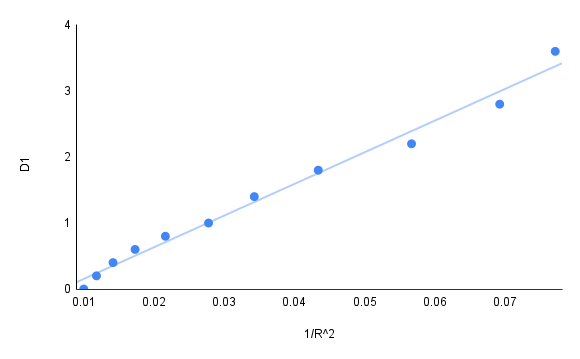
\includegraphics[width=0.8\textwidth]{Lab 2 Graph.png}
    \caption{The graph above shows the plotted points of $1/R^2$ and $D_1$,
    while also showing the line of best fit. As displayed here, there seems to be a positive
    linear trend in the relationship between the variables.}
    \label{fig:graph}
\end{figure}

\pagebreak
\section{Straight Line}
As shown in the graph above, the data plotted for $1/R^2$ vs. $D1$ fits a straight line very well.
It essentially demonstrates that $D_1 \propto 1/R^2$, since our $1/R^2$ increases as our brass ball
approaches our pith ball (hence increasing $D_1$). We also know from Coulombs Law, that our electrostatic force
$F_e = \frac{kq_1q_2}{r^2}$, and so $F_e \propto (1/r^2) = (1/R^2)$ and $D_1 \propto (1/R^2)$. \\

\noindent Therefore, we can conclude that as our $D_1$ increases (our brass ball gets closer to the pith ball),
the electrostatic force also increases.

\section{Charge Dissipation}
If a noticable amount of charge was dissipated during our experiment, it would show in our graph.
Let's firstly assume that is is our brass ball that loses its charge. Then, it would no longer push the pith ball further away since there is no repuslion force,
and our resulting graph would demonstrate a steep drop since our $D_1$ would decrease with our $D_2$ staying the same. \\ 

\noindent Now, if our pith ball charge dissipated, then again the repulsion force would not be present, and our pith ball would not push itself away from our brass ball,
and so we have the same result as above, with our graph demonstrating a steep drop.

\renewcommand{\refname}{References and Acknowledgements}
\begin{thebibliography}{9}
    \bibitem{labmanual} 
    Department of Physics. \textit{PHYS 126 Lab Manual}. University of Alberta, 2025.

    \bibitem{person}
    TA assisted with the lab, and provided guidance on the data collection and analysis.

    \bibitem{person}
    Lab partner Morgan Reinhart assisted with the data collection and analysis.
    
\end{thebibliography}
\end{document}